\begin{figure}[H]
\centering
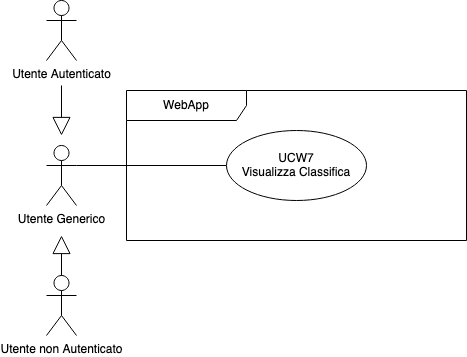
\includegraphics[scale=0.5]{UC_images/UCW7.png}
\caption{UCW7 - Visualizza Classifica}
\end{figure}
\begin{center}
\end{center}
\begin{itemize}
	\item \textbf{Descrizione}: L'utente generico visualizza la classifica dei locali presenti sulla piattaforma Sweeat.
    \item \textbf{Attore primario}: Utente generico.
    \item \textbf{Precondizione}: L’utente si trova all’interno della piattaforma Sweeat.
    \item \textbf{Postcondizione}: L’utente visualizza a schermo la classifica dei migliori locali gastronomici prodotta dal sistema, senza alcun filtro applicato e con i parametri di ordinamento di default.
    \item \textbf{Scenario principale}: 
    \begin{enumerate}
        \item Un utente generico accede al sistema;
        \item L’utente effettua una ricerca;
        \item L'utente visualizza la classifica con i risultati.
    \end{enumerate}
	\item \textbf{Sottocasi}:
	\begin{enumerate}
	\item L'utente visualizza un singolo locale (UCW 7.1 \S{3.8.1}).
	\end{enumerate}    
\end{itemize}

\begin{figure}[H]
    \centering
        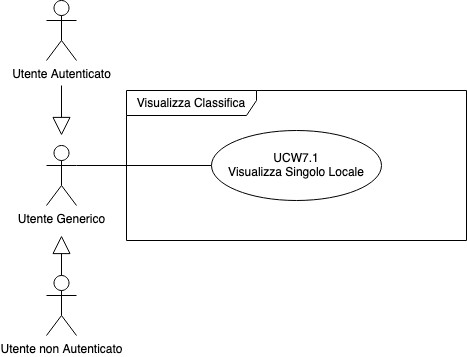
\includegraphics[scale=0.5]{UC_images/UCW7-x.png}
        \caption{Sottocasi UCW7.1}
\end{figure}

\subsubsection{UCW7.1 - Visualizza singolo locale}
\begin{itemize}
	\item \textbf{Descrizione}: L'utente generico visualizza un singolo locale dalla pagina dei risultati.
    \item \textbf{Attore primario}: Utente generico.
    \item \textbf{Precondizione}: L’utente si trova nella pagina dei risultati della piattaforma Sweeat.
    \item \textbf{Postcondizione}: L’utente visualizza il locale di suo interesse.
    \item \textbf{Scenario principale}: 
    \begin{enumerate}
        \item Un utente generico accede al sistema;
        \item L’utente effettua una ricerca;
        \item L'utente visualizza la classifica con i risultati;
        \item L'utente sceglie di visualizzare un locale specifico presente nella lista dei risultati.
    \end{enumerate}
	\item \textbf{Sottocasi}:
    \begin{enumerate}
	\item Visualizza informazioni locale (UCW7.1.1 \S{3.8.2}),
	\item Visualizza punteggi locale (UCW7.1.2 \S{3.8.3}), 
	\item Visualizza link locale (UCW7.1.3 \S{3.8.4}).	
	\end{enumerate}    
\end{itemize}

\begin{figure}[H]
    \centering
        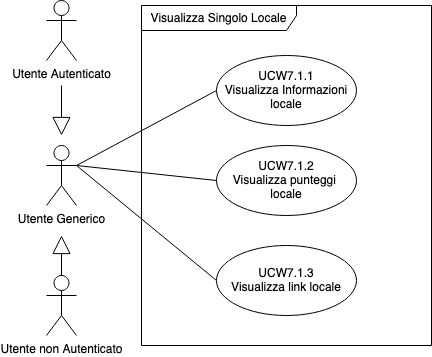
\includegraphics[scale=0.5]{UC_images/UCW7-1-x.png}
        \caption{Sottocasi UCW7.1}
\end{figure}

\subsubsection{UCW7.1.1 - Visualizza informazioni locale}
\begin{itemize}
	\item \textbf{Descrizione}: L'utente generico visualizza le informazioni di un singolo locale dalla pagina dei risultati.
    \item \textbf{Attore primario}: Utente generico.
    \item \textbf{Precondizione}: L’utente si trova nella pagina dei risultati della piattaforma Sweeat.
    \item \textbf{Postcondizione}: L’utente visualizza le informazioni del locale di suo interesse.
    \item \textbf{Scenario principale}: 
    \begin{enumerate}
        \item Un utente generico accede al sistema;
        \item L’utente effettua una ricerca;
        \item L'utente visualizza la classifica con i risultati;
        \item L'utente sceglie di visualizzare le informazioni relative ad uno specifico locale presente nella lista dei risultati.
    \end{enumerate}
	\item \textbf{Sottocasi}:
    \begin{enumerate}
	\item Visualizza nome locale (UCW7.1.1.1 \S{3.8.3}),
	\item Visualizza categoria locale (UCW7.1.1.2 \S{3.8.4}), 
	\item Visualizza immagine copertina (UCW7.1.1.3 \S{3.8.5}).	
	\item Visualizza numero di telefono locale (UCW7.1.1.4 \S{3.8.6}).	
	\item Visualizza orari di apertura locale (UCW7.1.1.5 \S{3.8.7}).	
	\item Visualizza giorni di apertura locale (UCW7.1.1.6 \S{3.8.8}).			
	\end{enumerate}    
\end{itemize}

\begin{figure}[H]
    \centering
        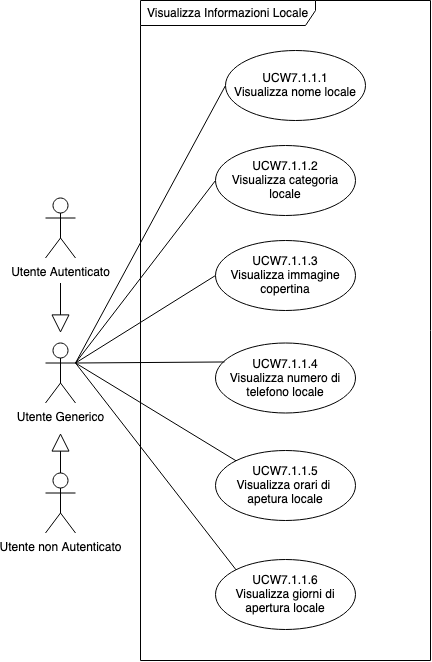
\includegraphics[scale=0.5]{UC_images/UCW7-1-1-x.png}
        \caption{Sottocasi UCW7.1.1}
\end{figure}

\subsubsection{UCW7.1.1.1 - Visualizza nome locale}
\begin{itemize}
	\item \textbf{Descrizione}: L'utente generico visualizza il nome del locale di suo interesse presente nella classifica.
    \item \textbf{Attore primario}: Utente generico.
    \item \textbf{Precondizione}: L’utente si trova nella pagina dei risultati della piattaforma Sweeat e visualizza le informazioni relative ad uno specifico locale.
    \item \textbf{Postcondizione}: L’utente visualizza il nome del locale di suo interesse presente nella classifica.
    \item \textbf{Scenario principale}: 
    \begin{enumerate}
        \item Un utente generico accede al sistema;
        \item L’utente effettua una ricerca;
        \item L'utente visualizza la classifica con i risultati;
        \item L'utente sceglie di visualizzare le informazioni relative ad uno specifico locale presente nella lista dei risultati;
        \item L'utente visualizza il nome del locale di suo interesse.
    \end{enumerate}
\end{itemize}

\subsubsection{UCW7.1.1.2 - Visualizza categoria locale}
\begin{itemize}
	\item \textbf{Descrizione}: L'utente generico visualizza la categoria a cui appartiene il locale di suo interesse presente nella classifica.
    \item \textbf{Attore primario}: Utente generico.
    \item \textbf{Precondizione}: L’utente si trova nella pagina dei risultati della piattaforma Sweeat e visualizza le informazioni relative ad uno specifico locale.
    \item \textbf{Postcondizione}: L’utente visualizza la categoria associata al locale di suo interesse presente nella classifica.
    \item \textbf{Scenario principale}: 
    \begin{enumerate}
        \item Un utente generico accede al sistema;
        \item L’utente effettua una ricerca;
        \item L'utente visualizza la classifica con i risultati;
        \item L'utente sceglie di visualizzare le informazioni relative ad uno specifico locale presente nella lista dei risultati;
        \item L'utente visualizza la categoria del locale di suo interesse.
    \end{enumerate}
\end{itemize}

\subsubsection{UCW7.1.1.3 - Visualizza immagine copertina}
\begin{itemize}
	\item \textbf{Descrizione}: L'utente generico visualizza l'immagine di copertina che rappresenta il locale di suo interesse presente nella classifica.
    \item \textbf{Attore primario}: Utente generico.
    \item \textbf{Precondizione}: L’utente si trova nella pagina dei risultati della piattaforma Sweeat e visualizza le informazioni relative ad uno specifico locale.
    \item \textbf{Postcondizione}: L’utente visualizza la foto associata al locale di suo interesse presente nella classifica.
    \item \textbf{Scenario principale}: 
    \begin{enumerate}
        \item Un utente generico accede al sistema;
        \item L’utente effettua una ricerca;
        \item L'utente visualizza la classifica con i risultati;
        \item L'utente sceglie di visualizzare le informazioni relative ad uno specifico locale presente nella lista dei risultati;
        \item L'utente visualizza la foto di copertina del locale di suo interesse.
    \end{enumerate}
\end{itemize}

\subsubsection{UCW7.1.1.4 - Visualizza numero di telefono locale}
\begin{itemize}
	\item \textbf{Descrizione}: L'utente generico visualizza il numero di telefono del locale di suo interesse presente nella classifica.
    \item \textbf{Attore primario}: Utente generico.
    \item \textbf{Precondizione}: L’utente si trova nella pagina dei risultati della piattaforma Sweeat e visualizza le informazioni relative ad uno specifico locale.
    \item \textbf{Postcondizione}: L’utente visualizza il numero di telefono del locale di suo interesse presente nella classifica.
    \item \textbf{Scenario principale}: 
    \begin{enumerate}
        \item Un utente generico accede al sistema;
        \item L’utente effettua una ricerca;
        \item L'utente visualizza la classifica con i risultati;
        \item L'utente sceglie di visualizzare le informazioni relative ad uno specifico locale presente nella lista dei risultati;
        \item L'utente visualizza il numero di telefono del locale di suo interesse.
    \end{enumerate}
\end{itemize}

\subsubsection{UCW7.1.1.5 - Visualizza orari di apertura locale}
\begin{itemize}
	\item \textbf{Descrizione}: L'utente generico visualizza gli orari di apertura del locale di suo interesse presente nella classifica.
    \item \textbf{Attore primario}: Utente generico.
    \item \textbf{Precondizione}: L’utente si trova nella pagina dei risultati della piattaforma Sweeat e visualizza le informazioni relative ad uno specifico locale.
    \item \textbf{Postcondizione}: L’utente visualizza gli orari di apertura del locale di suo interesse presente nella classifica.
    \item \textbf{Scenario principale}: 
    \begin{enumerate}
        \item Un utente generico accede al sistema;
        \item L’utente effettua una ricerca;
        \item L'utente visualizza la classifica con i risultati;
        \item L'utente sceglie di visualizzare le informazioni relative ad uno specifico locale presente nella lista dei risultati;
        \item L'utente visualizza gli orari di apertura del locale di suo interesse.
    \end{enumerate}
\end{itemize}

\subsubsection{UCW7.1.1.6 - Visualizza giorni di apertura locale}
\begin{itemize}
	\item \textbf{Descrizione}: L'utente generico visualizza i giorni di apertura del locale di suo interesse presente nella classifica.
    \item \textbf{Attore primario}: Utente generico.
    \item \textbf{Precondizione}: L’utente si trova nella pagina dei risultati della piattaforma Sweeat e visualizza le informazioni relative ad uno specifico locale.
    \item \textbf{Postcondizione}: L’utente visualizza i giorni di apertura del locale di suo interesse presente nella classifica.
    \item \textbf{Scenario principale}: 
    \begin{enumerate}
        \item Un utente generico accede al sistema;
        \item L’utente effettua una ricerca;
        \item L'utente visualizza la classifica con i risultati;
        \item L'utente sceglie di visualizzare le informazioni relative ad uno specifico locale presente nella lista dei risultati;
        \item L'utente visualizza i giorni di apertura del locale di suo interesse.
    \end{enumerate}
\end{itemize}

\subsubsection{UCW7.1.2 - Visualizza Punteggi Locale}
\begin{itemize}
	\item \textbf{Descrizione}: L'utente generico visualizza i punteggi totali del locale presente nella classifica. Il punteggio totale è ottenuto tenendo conto dei punteggi relativi a: foto, testi ed emoji.
    \item \textbf{Attore primario}: Utente generico.
    \item \textbf{Precondizione}: L’utente si trova nella pagina dei risultati della piattaforma Sweeat e visualizza le informazioni relative ad uno specifico locale.
    \item \textbf{Postcondizione}: L’utente visualizza i punteggi associati al locale di suo interesse presente nella classifica.
    \item \textbf{Scenario principale}: 
    \begin{enumerate}
        \item Un utente generico accede al sistema;
        \item L’utente effettua una ricerca;
        \item L'utente visualizza la classifica con i risultati;
        \item L'utente sceglie di visualizzare le informazioni relative ad uno specifico locale presente nella lista dei risultati;
        \item L'utente visualizza i vari punteggi associati al locale di suo interesse.
    \end{enumerate}
    \item \textbf{Sottocasi}:
    \begin{enumerate}
	\item Visualizza punteggio totale (UCW7.1.2.1 \S{3.8.10}),
	\item Visualizza punteggio foto (UCW7.1.2.2 \S{3.8.11}), 
	\item Visualizza punteggio testi (UCW7.1.2.3 \S{3.8.11}),
	\item Visualizza punteggio emoji (UCW7.1.2.4 \S{3.8.12}).		
	\end{enumerate} 
\end{itemize}

\begin{figure}[H]
    \centering
        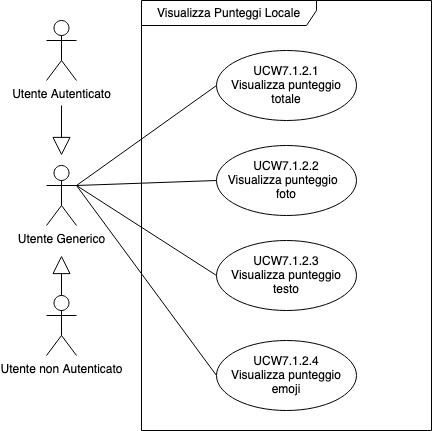
\includegraphics[scale=0.5]{UC_images/UCW7-1-2-x.png}
        \caption{Sottocasi UCW7.1.2}
\end{figure}

\subsubsection{UCW7.1.2.1 - Visualizza punteggio totale}
\begin{itemize}
	\item \textbf{Descrizione}: L'utente generico visualizza il punteggio totale associato al locale di suo interesse presente nella classifica.
    \item \textbf{Attore primario}: Utente generico.
    \item \textbf{Precondizione}: L’utente si trova nella pagina dei risultati della piattaforma Sweeat e visualizza le informazioni relative ad uno specifico locale.
    \item \textbf{Postcondizione}: L’utente visualizza il punteggio totale del locale di suo interesse presente nella classifica.
    \item \textbf{Scenario principale}: 
    \begin{enumerate}
        \item Un utente generico accede al sistema;
        \item L’utente effettua una ricerca;
        \item L'utente visualizza la classifica con i risultati;
        \item L'utente sceglie di visualizzare le informazioni relative ad uno specifico locale presente nella lista dei risultati;
        \item L'utente visualizza il punteggio totale del locale di suo interesse.
    \end{enumerate}
\end{itemize}

\subsubsection{UCW7.1.2.2 - Visualizza punteggio foto}
\begin{itemize}
	\item \textbf{Descrizione}: L'utente generico visualizza il punteggio delle foto pubblicate sui social associate al locale di suo interesse presente nella classifica.
    \item \textbf{Attore primario}: Utente generico.
    \item \textbf{Precondizione}: L’utente si trova nella pagina dei risultati della piattaforma Sweeat e visualizza le informazioni relative ad uno specifico locale.
    \item \textbf{Postcondizione}: L’utente visualizza il punteggio relativo alle foto pubblicate sui social relative al locale di suo interesse presente nella classifica.
    \item \textbf{Scenario principale}: 
    \begin{enumerate}
        \item Un utente generico accede al sistema;
        \item L’utente effettua una ricerca;
        \item L'utente visualizza la classifica con i risultati;
        \item L'utente sceglie di visualizzare le informazioni relative ad uno specifico locale presente nella lista dei risultati;
        \item L'utente visualizza il punteggio delle foto pubblicate sui social relative al locale di suo interesse.
    \end{enumerate}
\end{itemize}

\subsubsection{UCW7.1.2.3 - Visualizza punteggio testo}
\begin{itemize}
	\item \textbf{Descrizione}: L'utente generico visualizza il punteggio dei testi dei post pubblicati sui social associati al locale di suo interesse presente nella classifica.
    \item \textbf{Attore primario}: Utente generico.
    \item \textbf{Precondizione}: L’utente si trova nella pagina dei risultati della piattaforma Sweeat e visualizza le informazioni relative ad uno specifico locale.
    \item \textbf{Postcondizione}: L’utente visualizza il punteggio dei testi dei post associati al locale di suo interesse presente nella classifica.
    \item \textbf{Scenario principale}: 
    \begin{enumerate}
        \item Un utente generico accede al sistema;
        \item L’utente effettua una ricerca;
        \item L'utente visualizza la classifica con i risultati;
        \item L'utente sceglie di visualizzare le informazioni relative ad uno specifico locale presente nella lista dei risultati;
        \item L'utente visualizza il punteggio dei testi dei post pubblicati sui social relativi al locale di suo interesse.
    \end{enumerate}
\end{itemize}

\subsubsection{UCW7.1.2.4 - Visualizza punteggio emoji}
\begin{itemize}
	\item \textbf{Descrizione}: L'utente generico visualizza il punteggio delle emoji dei testi dei post pubblicati sui social associati al locale di suo interesse presente nella classifica.
    \item \textbf{Attore primario}: Utente generico.
    \item \textbf{Precondizione}: L’utente si trova nella pagina dei risultati della piattaforma Sweeat e visualizza le informazioni relative ad uno specifico locale.
    \item \textbf{Postcondizione}: L’utente visualizza il punteggio delle emoji dei testi dei post associate al locale di suo interesse presente nella classifica.
    \item \textbf{Scenario principale}: 
    \begin{enumerate}
        \item Un utente generico accede al sistema;
        \item L’utente effettua una ricerca;
        \item L'utente visualizza la classifica con i risultati;
        \item L'utente sceglie di visualizzare le informazioni relative ad uno specifico locale presente nella lista dei risultati;
        \item L'utente visualizza il punteggio delle emoji dei testi dei post pubblicati sui social del locale di suo interesse.
    \end{enumerate}
\end{itemize}

\subsubsection{UCW7.1.3 - Visualizza Link Locale}
\begin{itemize}
	\item \textbf{Descrizione}: L'utente generico visualizza i link del locale di suo interesse dalla pagina dei risultati.
    \item \textbf{Attore primario}: Utente generico.
    \item \textbf{Precondizione}: L’utente si trova nella pagina dei risultati della piattaforma Sweeat e visualizza le informazioni relative ad uno specifico locale.
    \item \textbf{Postcondizione}: L’utente visualizza i link del locale di suo interesse.
    \item \textbf{Scenario principale}: 
    \begin{enumerate}
        \item Un utente generico accede al sistema;
        \item L’utente effettua una ricerca;
        \item L'utente visualizza la classifica con i risultati;
        \item L'utente sceglie di visualizzare i link di uno specifico locale presente nella lista dei risultati.
    \end{enumerate}
	\item \textbf{Sottocasi}:
    \begin{enumerate}
	\item Visualizza informazioni locale (UCW7.1.3.1 \S{3.8.15}),
	\item Visualizza punteggi locale (UCW7.1.3.2 \S{3.8.16}), 
	\end{enumerate}    
\end{itemize}

\begin{figure}[H]
    \centering
        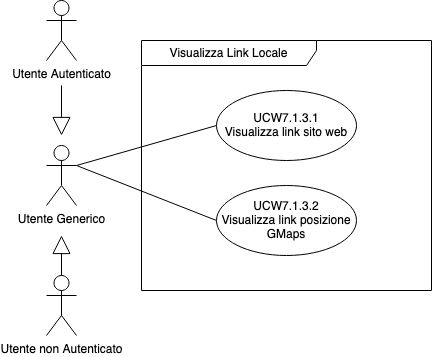
\includegraphics[scale=0.5]{UC_images/UCW7-1-3-x.png}
        \caption{Sottocasi UCW7.1.3}
\end{figure}

\subsubsection{UCW7.1.3.1 - Visualizza link sito web}
\begin{itemize}
	\item \textbf{Descrizione}: L'utente generico visualizza il link del sito web del locale di suo interesse presente nella pagina dei risultati.
    \item \textbf{Attore primario}: Utente generico.
    \item \textbf{Precondizione}: L’utente si trova nella pagina dei risultati della piattaforma Sweeat e visualizza le informazioni relative ad uno specifico locale.
    \item \textbf{Postcondizione}: L’utente visualizza il link al sito web del locale di suo interesse presente nella classifica.
    \item \textbf{Scenario principale}: 
    \begin{enumerate}
        \item Un utente generico accede al sistema;
        \item L’utente effettua una ricerca;
        \item L'utente visualizza la classifica con i risultati;
        \item L'utente sceglie di visualizzare le informazioni relative ad uno specifico locale presente nella lista dei risultati;
        \item L'utente visualizza il link al sito web del locale di suo interesse.
    \end{enumerate}
\end{itemize}

\subsubsection{UCW7.1.3.2 - Visualizza link posizione GMaps}
\begin{itemize}
	\item \textbf{Descrizione}: L'utente generico visualizza il link alla posizione su Google Maps del locale di suo interesse presente nella pagina dei risultati.
    \item \textbf{Attore primario}: Utente generico.
    \item \textbf{Precondizione}: L’utente si trova nella pagina dei risultati della piattaforma Sweeat e visualizza le informazioni relative ad uno specifico locale.
    \item \textbf{Postcondizione}: L’utente visualizza il link alla posizione su Google Maps del locale di suo interesse presente nella classifica.
    \item \textbf{Scenario principale}: 
    \begin{enumerate}
        \item Un utente generico accede al sistema;
        \item L’utente effettua una ricerca;
        \item L'utente visualizza la classifica con i risultati;
        \item L'utente sceglie di visualizzare le informazioni relative ad uno specifico locale presente nella lista dei risultati;
        \item L'utente visualizza il link alla posizione su Google Maps del locale di suo interesse.
    \end{enumerate}
\end{itemize}